\ProvidesFile{chapters/ch-Motivation_Theory.tex}

\chapter{MOTIVATION AND THEORETICAL OVERVIEW}
\label{Motivation_and_Theoretical_Overview}

\section{Reductionism and a Brief History of Particle Physics}
The reductionist approach to understanding the physical universe, by breaking it down to its smallest constituents and studying the interactions between them, is a central strategy of natural philosophy and the scientific method.
Well before there was evidence of the discreteness of matter, and despite human senses suggesting its continuity, ancient Greek philosophers Democritus and Leucippus introduced the concept of the atom as the fundamental building block of matter in the fifth century B.C.~\cite{sep-atomism-ancient}.
The atomic theory of the ancient Greeks sought to reduce components of the cosmos to matter and empty space, propose that the fundamental constituents of matter were indivisible, and provide a natural explanation for the diversity of matter as resulting from atoms of different properties forming complex arrangements.
This early reductionist philosophy was remarkably ahead of its time, and although ancient atomic theory and its concepts fell into obscurity after being rejected by later Greek philosophers, they were rediscovered by Enlightenment scientists in the early nineteenth century and laid the foundation for modern atomic theory, which forms the basis for understanding the structure of matter and the nature of chemical reactions.

Unprecedented progress in the field of particle physics has been made in the past two centuries following the adoption of the reductionist approach.
After discovering periodic trends, Mendeleev published the first version of the periodic table in 1869~\cite{mendeleev1869relationship}, which organized chemical elements in a tabular arrangement based on patterns of chemical properties and atomic weight.
By the end of the nineteenth century, with the discoveries of the electron ($e$) by Thomson in 1897~\cite{thomson1897xl} and nuclear radioactivity by Becquerel in 1896~\cite{becquerel1896radiations}, atoms were understood to not be indivisible and indestructible, and therefore could not be elementary constituents of matter.
In the early twentieth century, Moseley revised the periodic table of elements after discovering atomic number~\cite{Egdell2020}, and this revision established a more accurate and consistent periodic table that led to a better understanding of the electron structure of atoms.
Around the same time, Rutherford experimentally discovered the atomic nucleus~\cite{rutherford1911lxxix} and formulated the concept of the proton ($p$).
Some years later, to account for the missing mass discrepancy between measurements of atomic weight and atomic number, he also theorized the existence of neutrons.
With the discovery of the neutron ($n$) in 1932 by Chadwick~\cite{chadwick1932possible}, for a time it was thought that protons, neutrons, and electrons constituted fundamental particles.

The development of a quantum mechanical framework in the twentieth century provided a deeper understanding of the behavior of atomic and subatomic particles that helped to illuminate previously unexplained phenomena such as atomic spectra and nuclear radioactivity.
In the 1930s, Fermi formulated a theoretical framework that described beta decay as the result of the weak interaction between subatomic protons, neutrons, and electrons~\cite{Wilson:1968pwx}.
The development of the quantum field theory of electrodynamics (QED), led by Schwinger~\cite{PhysRev.74.1439} and Feynman~\cite{PhysRev.76.769} in the 1940s and 1950s, provided a complete theoretical quantum framework for describing electromagnetism, which is responsible for phenomena such as electricity and light.
With the development of cosmic ray experiments in the 1940s and particle accelerator experiments in the 1950s, an extensive ``zoo'' of subatomic and subnuclear particles were discovered.
The formulation of the quark model by Gell-Mann in 1964~\cite{GELLMANN1964214}, and the development of quantum field theory of chromodynamics (QCD), elucidated that protons, neutrons, and many other species in the particle zoo did not constitute fundamental particles, but instead were composed of combinations of elementary quarks bound together by a strong nuclear force.

\section{The Standard Model of Particle Physics}
The Standard Model (SM) of particle physics (summarized in figure~\ref{Standard_Model}), developed through the 1960's and early 1970's, reduced the complex and diverse behavior of all atomic and subatomic particles to the elementary particles and the fundamental interactions between them. 
The SM is a quantum field theory (QFT), defined mathematically by the local gauge symmetry group $SU(3) \otimes SU(2) \otimes U(1)$, that incorporates the strong, weak, and electromagnetic interactions~\cite{GLASHOW1961579},~\cite{PhysRevLett.19.1264},~\cite{doi:10.1142/9789812795915_0034},~\cite{HIGGS1964132},~\cite{PhysRevLett.13.508},~\cite{PhysRevLett.13.321},~\cite{PhysRevLett.30.1343}.
A field is an entity described by a Lagrangian density ($\mathcal{L}$), defined over all space-time, that is able to produce quanta when excited.
Elementary particles (described by their properties and quantum numbers spin, electric charge, color charge, and  weak isospin), are understood to be quantized energy excitations of fields, point-like objects that are truly indivisible without any substructure whatsoever, and are both creatable and destructible.
\begin{figure}[htb]
  \begin{center}
    \begin{tabular}{c}
        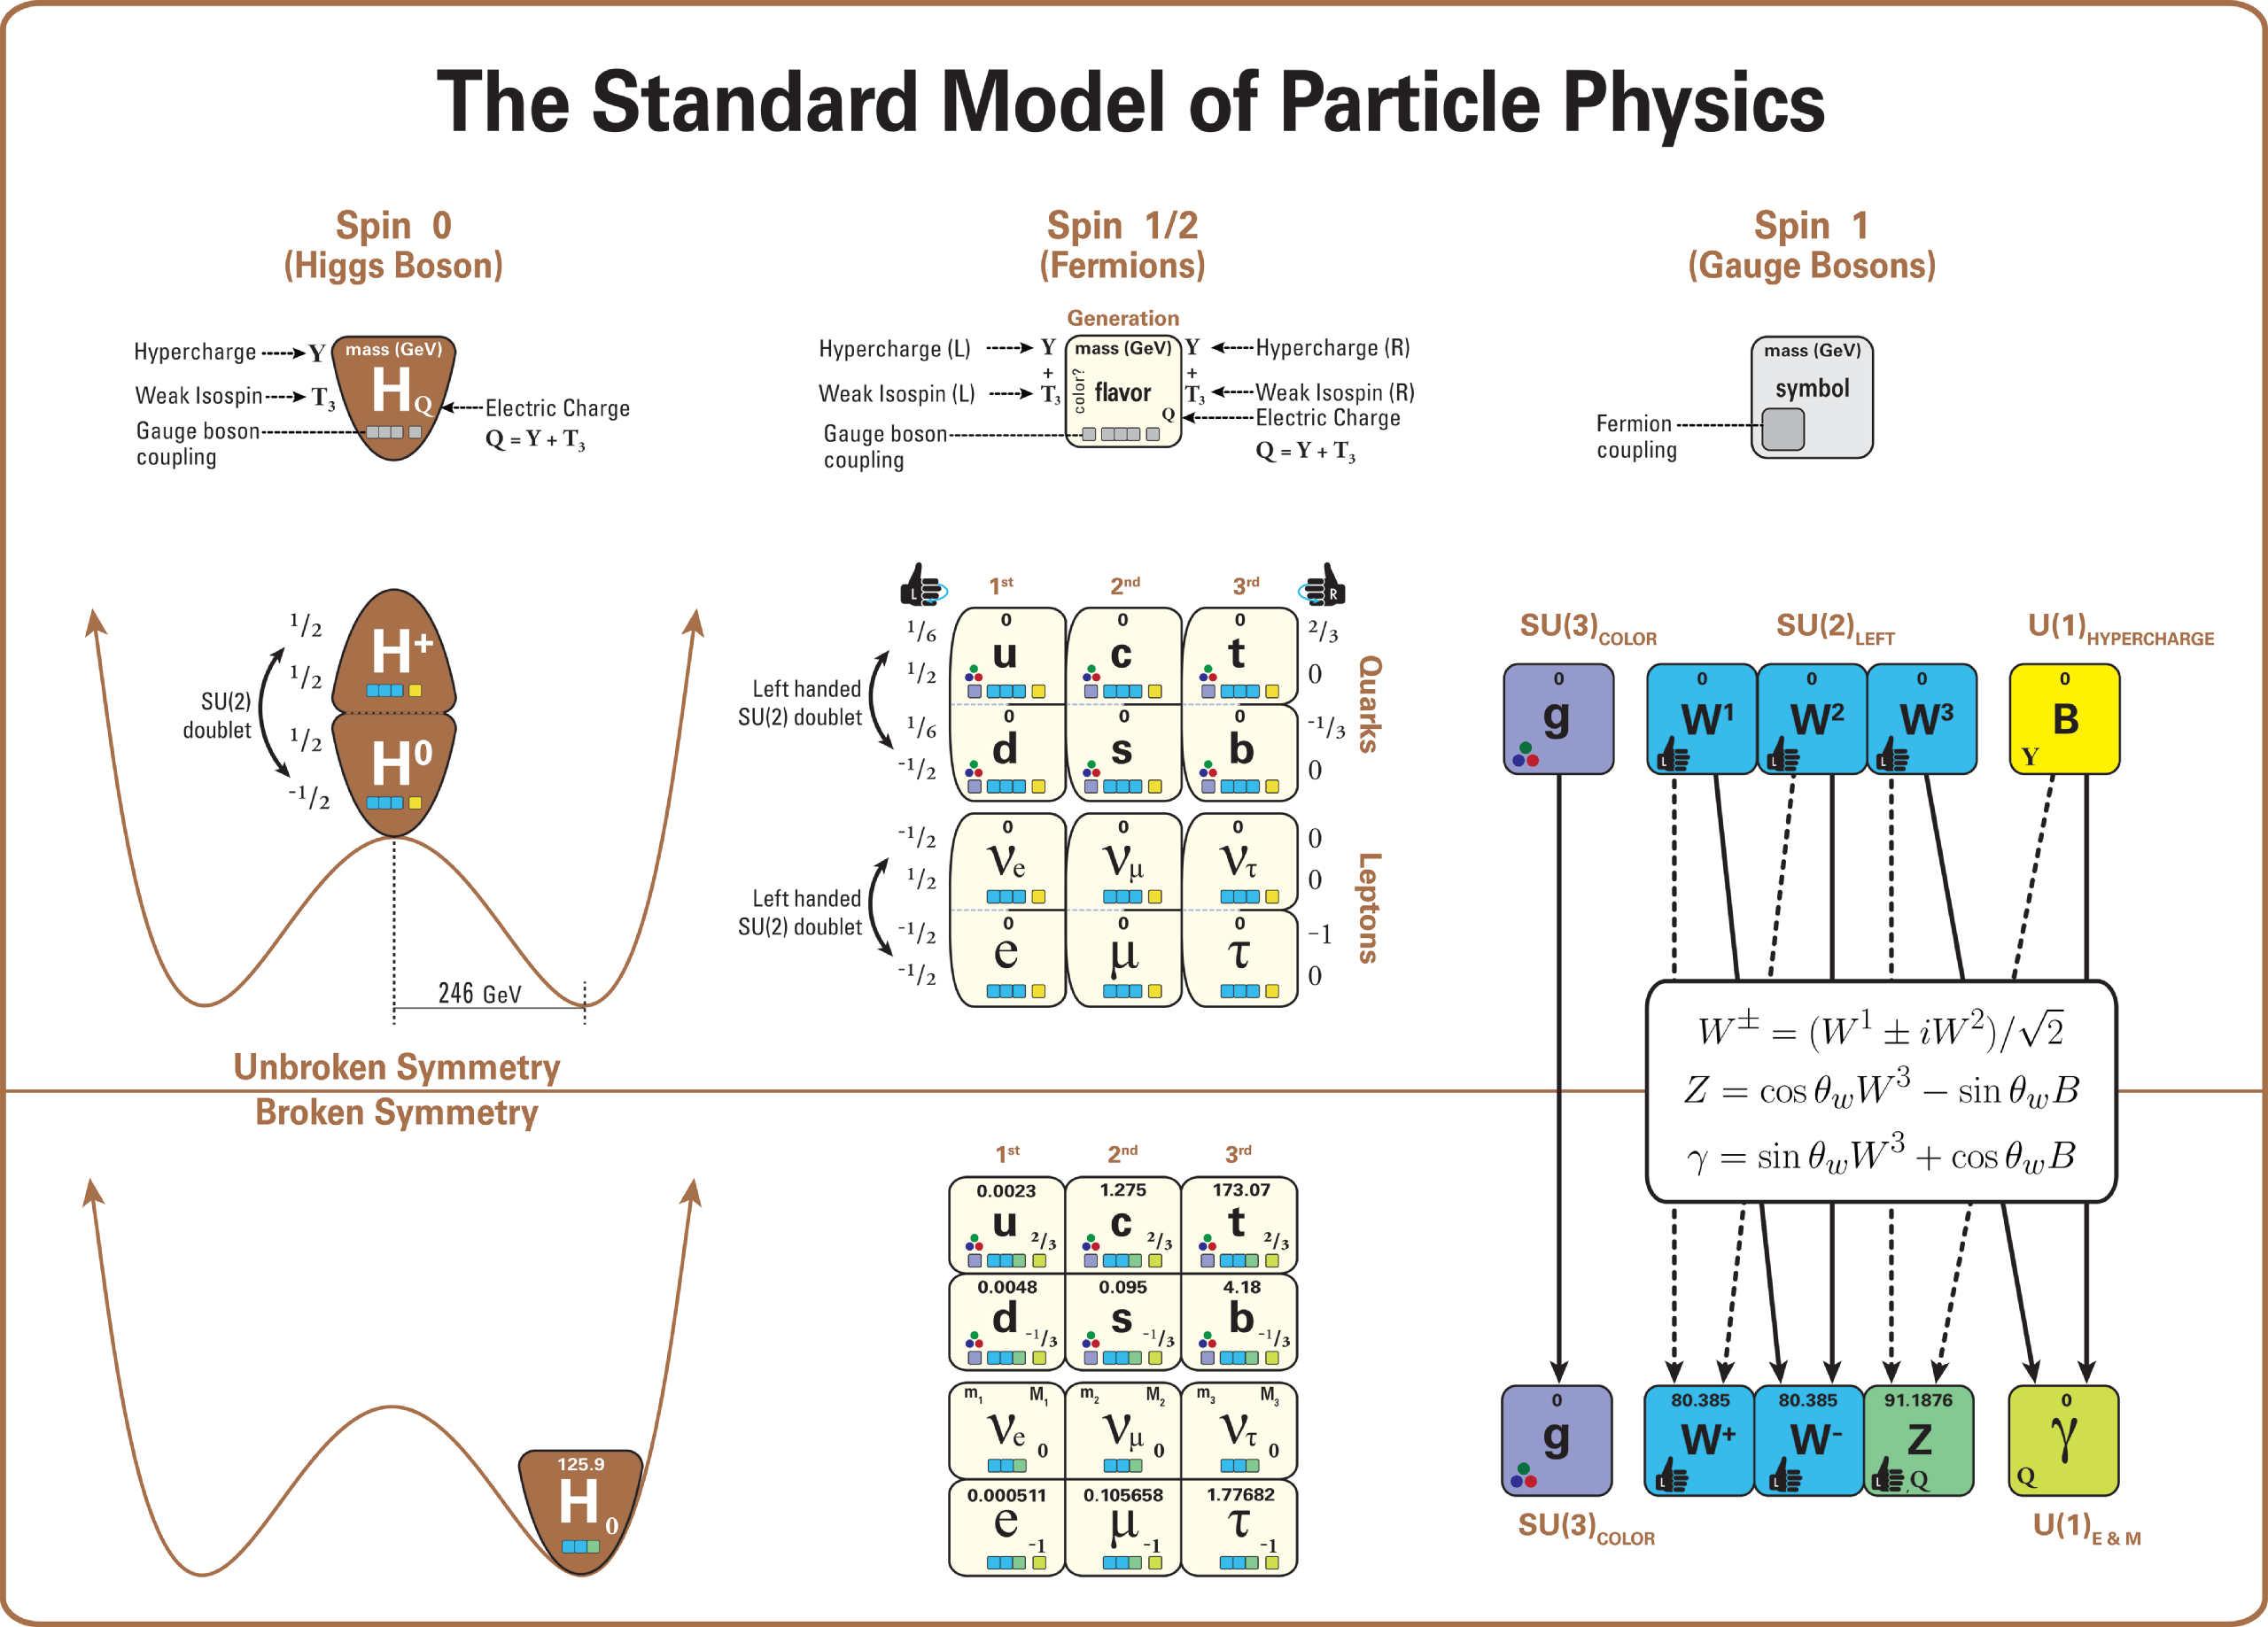
\includegraphics[width=1.00\textwidth]{fig_Theory/Standard_Model.png}
    \end{tabular}
    \caption{The Standard Model of Elementary Particle Physics~\cite{StandardModel}.
            }
    \label{Standard_Model}
  \end{center}
\end{figure}

\subsection{Fermions and Bosons}
In the SM, composite particles of matter are differentiated in terms of their constituent elementary particles of half-integer spin, called fermions, which are the building blocks of matter bound together by the exchange of fundamental, force-carrying particles of integer spin, called bosons. 

Fermions are further categorized into the quark and lepton subgroups.
Leptons and quarks carry electric charge ($Q$) and therefore participate in electromagnetic interactions.
Quarks additionally carry red ($R$), green ($G$), or blue ($B$) color charge, and so can also participate in strong interactions.
Because of this property and the nature of QCD, quarks cannot exist in isolation, but instead can only be observed confined to colorless bound states called hadrons.

There are three so-called ``generations'' of fermions, and each generation is composed of both a pair of leptons and a pair of quarks, resulting in a total of twelve fermions: six quarks and six leptons.
Fermions of higher generations are more massive than those of the previous generation.
The up ($u$) and down ($d$) quarks, together with the electron ($e$) and electron neutrino ($\nu_e$) leptons, compose the first generation of fermions.
Both protons and neutrons are composed of different combinations of three up and down quarks; therefore, virtually all atomic matter is composed of only first-generation fermions.
The second generation of fermions consists of the charm ($c$) and strange ($s$) quarks as well as the muon ($\mu$) and muon neutrino ($\nu_\mu$) leptons.
Finally, the third generation of fermions is composed of the top ($t$) and bottom ($b$) quarks (sometimes nicknamed truth and beauty), together with the tau ($\tau$) and tau neutrino ($\nu_\tau$) leptons.

The $e$, $\mu$, and $\tau$, referred to as "charged leptons", carry electric charge $Q = -1$, but the $\nu_e$, $\nu_\mu$, and $\nu_\tau$ neutrinos are electrically neutral.
The $u$, $c$, and $t$ quarks, referred to as "up-type," carry $Q = +\frac{2}{3}$, whereas the $d$, $c$, and $b$ quarks, referred to as "down-type," carry $Q = -\frac{1}{3}$.

Left-handed quarks and leptons additionally carry weak isospin ($I$ with third component $I_3$) and therefore participate in the weak interaction.
Left-handed charged leptons and down-type quarks carry $I_3 = +\frac{1}{2}$, while left-handed neutrinos and up-type quarks $I_3 = -\frac{1}{2}$.

Every fermion, denoted arbitrarily as $x$, has an anti-matter counterpart denoted $\bar{x}$, with the same mass as $x$, but sign-inverted quantum numbers.
The sign-inversions of red, green and blue color charges are anti-red (cyan), anti-green (magenta) and anti-blue (yellow), respectively.

The fundamental interactions of the SM are described by the exchange of force-mediating spin-$1$ vector bosons within the mathematical frameworks of gauge field theories.
These mediators arise from the gauge field group generators of the symmetry groups $U(1)$, $SU(2)$, and $SU(3)$.
The $U(1)$ group has one degree of freedom, and $SU(N)$ groups have $N^2 - 1$ degrees of freedom, so in total the SM has $12 = 1 + 3 + 8$ generators, corresponding to twelve gauge bosons.
The gauge coupling constants of the fundamental interactions are free parameters that are determined experimentally.
The SM also includes a spin-$0$ scalar boson associated with a scalar field responsible for the spontaneous symmetry breaking of the electroweak interaction and the generation of mass terms in the Lagrangian density for fermion fields.

\subsection{The Electromagnetic Interaction}
The photon ($\gamma$) is the massless and electrically neutral gauge boson that mediates the electromagnetic interaction between electrically charged particles.
The electromagnetic interaction is described by QED with gauge symmetry group $U(1)$.
The electromagnetic coupling, i.e. the fine structure constant ($\alpha_{EM} \approx \frac{1}{137}$ at low energies), is significantly small relative to unity.
For a given process, the momenta of mediating virtual photons depend on the energy scale, therefore the coupling constant "runs" and the interaction becomes stronger (but still significantly smaller than unity) at higher energy scales ($\alpha_{EM} \approx \frac{1}{128}$ at scale $m_Z \approx \SI{91.2}{\GeV}$).
As $\alpha_{EM} << 1$ even at high energy scales, perturbative power series expansions in $\alpha_{EM}$ have proven to be extremely effective at explaining experimental results with QED.
Despite only providing approximate predictions, this effectiveness has made QED one of the most well-tested and successful theories in physics.

\subsection{The Weak Interaction}
The $W^\pm$ and $Z$ are massive gauge bosons that mediate the weak interaction between fermions carrying weak isospin ($I$ with third component $I_3$).
$W^\pm$ carry $Q = \pm 1$, while $Z$ is electrically neutral.
Weak isospins of $I_3 = \pm 1$ ($I_3 = 0$) are carried by the $W^\pm$ ($Z$) bosons.
Their masses are $m_{W^\pm} \approx \SI{80.4}{\GeV}$ and $m_Z \approx \SI{91.2}{\GeV}$\footnote{In this dissertation, some quantities are expressed, when conventional, using the system of natural units. With this system, many expressions are simplified by setting the speed of light ($c$) and the reduced Planck's constant ($\hbar$) to unity and dimensional quantities can be expressed in units of energy or inverse energy. 
%For example, energy, momentum, and mass can be expressed in units of energy, while length and time can be expressed in units of inverse energy.
%In particle physics, energy is typically expressed in units of electronvolts ($\si{\eV}$), which is defined as the amount of kinetic energy gained by a single electron accelerated from rest through an electric potential difference of $\SI{1}{\V}$ in a vacuum. 
When these units are used, the standard dimensions can be recovered by appropriately multiplying or dividing by $c$ and $\hbar$.}, resulting in incredibly short lifetimes \sim$\SI{e-25}{\s}$. The short lifetimes limit the interaction ranges to extremely small scales, because the distance these bosons travel before decaying is very short.
The weak interaction is responsible for fermionic decay processes (such as nuclear radioactivity), is described in the SM by gauge symmetry group $SU(2)$, and is the only fundamental interaction that violates parity ($P$), charge conjugation parity ($CP$), and time-reversal ($T$) symmetries.
$Z$ bosons mediate the neutral weak interaction between same-flavor fermions, while $W^\pm$ bosons mediate the charged weak interaction between leptons of the same generation and can also flavor-mix quarks of different generations.
Information about the conversion probabilities of quark flavor changing weak decays is encoded in the four free parameters (3 mixing angles + 1 CP violating phase) of the Cabibbo-Kobayashi-Maskawa (CKM) matrix, which cannot be determined from underlying principles and are measured experimentally.

\subsection{The Strong Interaction}
Gluons ($g$) are massless gauge bosons that mediate the strong interaction between color-charged particles.
The strong interaction is described by QCD with gauge symmetry group $SU(3)_C$.
While quarks (anti-quarks) carry color (anti-color) charge, gluons uniquely carry both color and anti-color charge, and therefore gluons can interact with other gluons at trilinear and quartic self-interaction vertices.
There is a color octet of 8 different types of gluons, corresponding to 8 independent color state superpositions of the $3^2$ color/anti-color combinations.
One additional independent superposition exists mathematically, a color singlet carrying no color charge, but there is no experimental evidence for it and it is forbidden by $SU(3)_C$.

The strong coupling $\alpha_S$ runs vigorously as the energy scale decreases, i.e. the interaction strength between quarks becomes stronger the further the quarks are separated from each other.
This property of QCD results in color confinement~\cite{FRITZSCH1973365}, because before the energy between two separated quarks becomes arbitrarily large, a critical energy is reached for hadronization, in which the color-field lines snap and a new quark/anti-quark pair is created from the energy of the mediating gluon.
Hadrons are classified by the flavor combinations of their valence quarks, but because quark interactions are mediated by gluons that can interact with themselves and split into quark/anti-quark pairs, there also exists a sea of virtual quarks and gluons within hadrons.
Colorless flavor combinations of three valence quarks, such as protons and neutrons, are categorized as baryons, whereas colorless flavor combinations of one valence quark and one valence anti-quark, such as pions and kaons, are categorized as mesons.
Experimental evidence for colorless flavor combinations of five valence quarks, categorized as pentaquarks~\cite{PhysRevLett.115.072001}, and colorless flavor combinations of two valence quarks and two valence anti-quarks, categorized as tetraquarks~\cite{PhysRevLett.110.252002} have also been reported in recent years.
Of all known hadrons, only the proton appears to be stable; with a mean lifetime constrained to be at least $10^{34}$ years, proton decay has never been observed.

Another consequence of the running of $\alpha_S$ is asymptotic freedom~\cite{PhysRevLett.30.1343}.
At higher and higher energy scales, $\alpha_S$ asymptotically approaches zero (see figure~\ref{alphaS_running}), i.e. quarks and gluons behave more like free particles at high energies.
At sufficiently high energy scales, such as those in hard scattering processes at hadron collider experiments, perturbative power series expansions in $\alpha_S$ become effective at explaining experimental results with QCD.
For example, $\alpha_S(Q = m_Z =  \SI{91.2}{\GeV}) = 0.1171 \pm 0.0010$~\cite{PhysRevD.103.034028}.
\begin{figure}[htb]
  \begin{center}
    \begin{tabular}{c}
        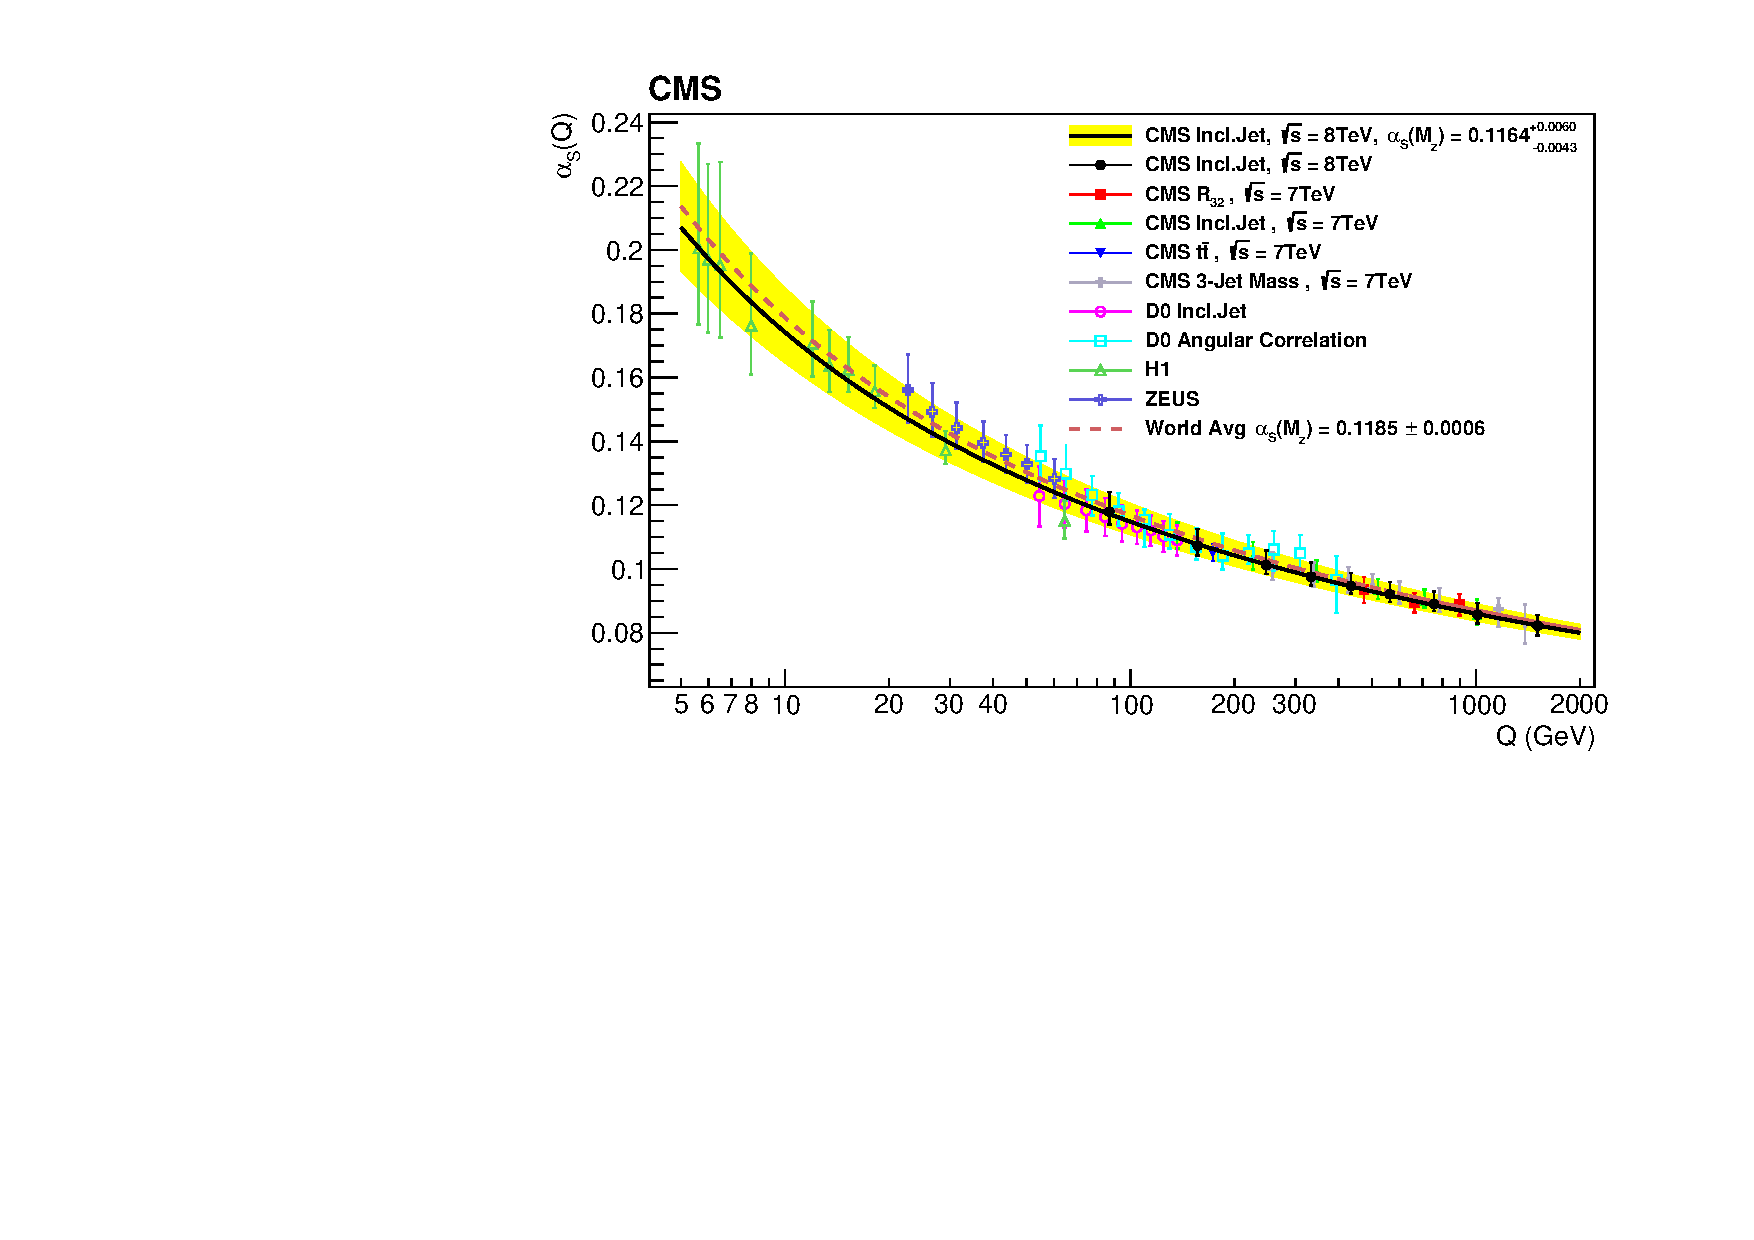
\includegraphics[width=0.65\textwidth]{fig_Theory/alphaS_running.pdf}
    \end{tabular}
    \caption{The running of the strong coupling constant $\alpha_S$ as a function of the momentum transfer $Q = \pT$~\cite{alphaS_running}.
            }
    \label{alphaS_running}
  \end{center}
\end{figure}

\subsection{The GWS Model, EWSB, and the BEH Mechanism}
At low energy scales, the electromagnetic and weak interactions are distinctly separate forces.
For energies beyond the electroweak transition scale \sim$\SI{160}{\GeV}$, electroweak theory unifies these two interactions into a single force described by a spontaneously broken quantum field with gauge symmetry group $SU(2)_L \otimes U(1)_Y$, generated by weak isospin carried by left-handed fermion doublets ($L$) and weak hypercharge ($Y$).
In the Glashow-Weinberg-Salam (GWS) model~\cite{GLASHOW1961579},~\cite{PhysRevLett.19.1264},~\cite{doi:10.1142/9789812795915_0034}, the $U(1)_Y$ group is generated by weak hypercharge and mediated by a massless $B^0$ boson, and the $SU(2)_L$ group is generated by weak isospin and mediated by massless $W^1$, $W^2$, and $W^3$ bosons.

In the SM, the $\gamma$, $Z$, and $W^\pm$ bosons arise from the Brout-Englert-Higgs (BEH) mechanism~\cite{HIGGS1964132},~\cite{PhysRevLett.13.508},~\cite{PhysRevLett.13.321} spontaneously inducing electroweak symmetry breaking (EWSB) in the GWS model.
Electric charge $Q = I_3 + \frac{1}{2} Y$ arises as a specific linear combination of weak isospin and hypercharge.
Electrically neutral $\gamma$ and $Z$ bosons arise from mixed states of the $B^0$ and $W^3$ bosons:
\begin{linenomath*}
\begin{align}
\left(\begin{array}{c}
\gamma \\
Z^0
\end{array}\right)=\left(\begin{array}{cc}
\cos \theta_{\mathrm{W}} & \sin \theta_{\mathrm{W}} \\
-\sin \theta_{\mathrm{W}} & \cos \theta_{\mathrm{W}}
\end{array}\right)\left(\begin{array}{c}
B \\
W_3
\end{array}\right)
\label{}
\end{align}
\end{linenomath*}
where $\theta_{\mathrm{W}}$ is the Weinberg weak mixing angle related to the gauge coupling strengths of $SU(2)$ and $U(1)$.
So the $Z$ boson couples to both left-handed and right-handed fermions via $W^3$ and $B^0$ respectively.
Electrically charged $W^\pm$ bosons arise from linear combinations of the $W^1$ and $W^2$ bosons:
\begin{linenomath*}
\begin{align}
W^{\pm}=\frac{1}{\sqrt{2}}\left(W_1 \mp i W_2\right).
\end{align}
\end{linenomath*}
and $W^\pm$ bosons couple to only left-handed fermions.

In the GWS model, local gauge symmetry prohibits mass terms in the Lagrangian for gauge bosons (Goldstone's theorem), but the $W^\pm$ and $Z$ bosons are experimentally known to have large masses.
To both resolve this discrepancy and induce EWSB, the BEH mechanism adds a complex scalar $SU(2)$ doublet field $\phi$ to the SM that permeates all of space:
\begin{linenomath*}
\begin{align}
\phi=\left(\begin{array}{l}
\phi^{+} \\
\phi^0
\end{array}\right)
\end{align}
\end{linenomath*}
with self-interacting potential energy:
\begin{linenomath*}
\begin{align}
V(\phi) = \mu^2 \phi^{\dagger} \phi + \lambda\left(\phi^{\dagger} \phi\right)^2 \quad \lambda >0
\end{align}
\end{linenomath*}
The BEH potential, colloquially referred to as a ``Mexican-hat'' potential for $\mu^2 < 0$, satisfies $SU(2) \otimes U(1)$.
The energy at the center of the potential is higher than at a ring of equivalent vacuum states with vacuum expectation energy $\langle 0 \vert \phi \vert 0 \rangle=\sqrt{\frac{-\mu^2}{2 \lambda}} \equiv \frac{v}{\sqrt{2}}$ that breaks the electroweak gauge symmetry.
By introducing the real and physical scalar Higgs field $H$, $\phi$ can be parameterized with an expansion around the vacuum expectation energy, and with a transformation to the unitary gauge:
\begin{linenomath*}
\begin{align}
\phi
=\frac{1}{\sqrt{2}}
\left(\begin{array}{l}
\omega_2/2 + i \omega_1/2 \\
v + H + i \omega_3/2
\end{array}\right)
= \frac{e^{\frac{ i \omega_j \cdot \sigma^j}{2v}}}{\sqrt{2}}
\left(\begin{array}{c}
0 \\
v+H
\end{array}\right)
\longrightarrow \phi^{\prime} = \frac{1}{\sqrt{2}}
\left(\begin{array}{c}
0 \\
v+H
\end{array}\right)
\end{align}
\end{linenomath*}
where $\sigma_j$ are the Pauli matrices.
Of the original four degrees of freedom in the complex scalar $SU(2)$ doublet field, the electrically charged $\omega_1$ and $\omega_2$ are absorbed to generate mass terms in the Lagrangian for the $W^\pm$ bosons $m_{W^\pm} = \frac{v}{2}$, while the electrically neutral $\omega_3$ is absorbed to generate mass for the $Z$ boson, such that $m_{W^\pm} = m_Z \cos \theta_{\mathrm{W}}$.
The remaining electrically neutral degree of freedom is split into $v$ and the new field $H$, with quantum numbers $I_3 = -\frac{1}{2}$ and $Y = +1$ ($Q = 0$), which mediates interactions between the fermions and the BEH field via the scalar Higgs ($H^0$) boson, endowing them with mass $m_f = \frac{v}{\sqrt{2}} y_f$ proportional to their Yukawa coupling $y_f$ and the vacuum expectation energy $v$.
The nine\footnote{The SM assumes the three neutrinos are massless, but it has been observed experimentally that neutrinos undergo flavor oscillations as they propagate through space, implying non-zero mass differences~\cite{PhysRevLett.81.1562}.} Yukawa couplings cannot be determined from any underlying principles and are free parameters that are determined experimentally.
The Higgs boson also acquires mass $m_H = v \sqrt{2 \lambda}$ through self-interaction with the BEH field.
Both $\mu$ and $\lambda$ are free parameters of the SM that determine $v \approx \SI{246}{\GeV}$ and $m_H \approx \SI{125}{\GeV}$.
The Higgs boson was experimentally discovered, in 2012 jointly by the CMS~\cite{201230} and ATLAS~\cite{20121} LHC experiments at CERN, with mass $m_H \approx \SI{125}{\GeV}$; Peter Higgs and François Englert received the 2013 Nobel Prize in Physics for their theoretical predictions, while Robert Brout passed away in 2011.

\subsection{Standard Model Lagrangian Density}
In summary, the notation for the SM Lagrangian density can be abbreviated into the following form:
\begin{linenomath*}
\begin{align}
\mathcal{L}_{SM} &= \mathcal{L}_{Yang-Mills} + \mathcal{L}_{Dirac} + \mathcal{L}_{Yukawa} + \mathcal{L}_{Higgs} \\
\mathcal{L}_{SM} &= -\frac{1}{4} F_{\mu \nu} F^{\mu \nu} + i\bar{\psi} \cancel{D} \psi+\text {h.c.} + \bar{\psi}_i y_{i j} \psi_j \phi+\text {h.c.} + \left \vert D_\mu \phi\right \vert^2 - V(\phi)
\end{align}
\end{linenomath*}
where the first term (Yang-Mills) describes the dynamics of the gauge fields responsible for the fundamental interactions, the second and third terms (Dirac) describe how these gauge fields interact with the fermion fields (with h.c. corresponding to the hermitian conjugate of the preceding term), the fourth and fifth terms (Yukawa) describe how the fermion fields obtain mass via interaction with the BEH field, the sixth and seventh terms (Higgs) describes the BEH potential and the interaction of the BEH field with the gauge fields.

\section{Beyond the Standard Model}
The SM is a central pillar of modern particle physics; many of its predictions have been confirmed by innumerable experiments to exquisite precision, and it is considered to be one of the most mature and successful theories in all of science.
Despite its success, there are a number of known physical phenomena that are not explained by the SM, and it is considered to be an effective theory up to some scale $\Lambda \approx \si{\TeV}$.
All theoretical and experimental investigations that are beyond the current understanding of the Standard Model of particle physics are collectively referred to as Beyond the Standard Model (BSM).

Following the example of electroweak unification, theoretical frameworks that aim to unify the strong and electroweak interactions into a single, unified force are referred to as Grand Unification Theories (GUT).
While the scale of electroweak unification is \sim$\SI{e2}{\GeV}$, the scale of grand unification is estimated to be \sim$\SI{e14}{\GeV} - \SI{e16}{\GeV}$.
Given the extreme energy requirements, it is unsurprising that no experimental evidence for GUT predictions has been found yet at energy scales accessible to modern particle accelerator experiments.

The theoretical explanation for the experimental observation of neutrino oscillations predicts that the neutrino masses are non-zero.
However, the SM predicts that neutrinos should be massless particles. 

The discovery of the Higgs boson with mass $m_H \approx \SI{125}{\GeV}$ has created an inconsistency in the SM known as the "Hierarchy Problem."
Assuming that the SM is valid up to some energy scale, virtual loop corrections to the Higgs boson mass generate quadratic divergences.
Calculating a predicted Higgs boson mass compatible with the observed value requires unnatural fine-tuning, highlighting the likelihood of New Physics (NP) between the electroweak scale and the Planck scale, i.e. the natural scale of quantum gravity.

Of the natural forces considered to be fundamental, only the gravitational interaction between massive objects is not described by the SM framework in a quantum field theory formulation.
A theory that reduces all four physical interactions into a single, unified theory is colloquially referred to as the ``Theory of Everything,'' and it is the holy grail of particle physics.
Einstein's general theory of relativity (GR)~\cite{einstein1915feldgleichungen} is a classical theory of gravitation that describes the force of gravity as resulting from the curvature of spacetime caused by the presence of massive objects.
All attempts to unify the SM and GR have failed, and the two are considered to be separate and incompatible theories.
A major focus of current theoretical physics research is centered around the formulation of a QFT that describes the gravitational interaction, but a common feature of these theories is that they are non-renormalizable.
Theories of quantum gravity predict the existence of a massless, spin-2 gauge boson dubbed the graviton.
Experimentally, however, gravity is \sim$10^{24}$ times weaker than the weak interaction, and the lack of experimental sensitivity makes it extremely difficult to verify the predictions of these theories.

There also are astrophysical and cosmological observed phenomena that are not explained by the SM.
For example, there is no explanation for the observed asymmetry between matter and anti-matter in the visible universe.
Based on the assumption that the universe started with equal quantities of matter and anti-matter, the conditions required for baryogenesis (i.e. the generation of a cosmological excess of baryons over anti-baryons) include baryon number violation, CP-violation, and charge conjugation symmetry ($C$) violation.
Sources of CP-violation in the SM via the weak interaction are not sufficient to account for the extreme asymmetry and baryon number is not violated whatsoever.
CP-violation via the strong interaction is mathematically allowed in the SM, but the relevant parameters have been inexplicably measured to be extremely small (strong CP problem).
Astronomical observations of gravitational lensing effects and in the velocity of rotation curves of spiral galaxies suggest that $85 \%$ of all observed matter in the universe is dark matter, an unknown form of matter that has its namesake in that it does not emit, absorb or reflect electromagnetic radiation, and thus can only be indirectly inferred through its gravitational effects on visible matter.
Although dedicated dark matter detection experiments exist that search for Weakly Interacting Massive Particles (WIMP), conclusive direct observation of dark matter WIMPs has not yet occurred.
Cosmological observations of galaxies also indicate that the expansion of space is accelerating.
The cause of this expansion is unknown, but it is attributed to an enigmatic form of energy, dubbed dark energy, that is thought to be responsible for $73 \%$ of the total energy density of the universe.

Many BSM extensions have been made that predict new elementary particles that, depending on their properties and stability, could explain dark matter.
Perhaps the most popular of these extensions is Supersymmetry (SUSY), which predicts the existence of superpartners for every fermion and boson in the SM by adding terms to the Lagrangian and make it symmetric with respect to matter and field-mediating particles.
SUSY can resolve the hierarchy problem by providing superpartner terms that cancel the quadratic divergences to the Higgs boson mass from heavy virtual particles.
Despite compelling arguments for why the predicted superpartners could be within reach of LHC experiments, the lack of experimental evidence for SUSY has led to a resurgence of interest in alternative BSM models to resolve these open questions.

SM Effective Field Theory (SMEFT) is a model-independent extension of the Standard Model which uses a systematic product expansion in terms of higher-dimensional operators to describe the effects of NP at higher energy scales~\cite{BUCHMULLER1986621}.  
Due to its agnostic construction, SMEFT allows for a broad range of possibilities for NP.
The SM, composed of mass dimension-2 and mass dimension-4 operators, is assumed to be an effective field theory that describes physical interactions up to some energy scale $\Lambda$.
The SMEFT Lagrangian is expanded as a power series in $\Lambda$, with the contributions beyond the SM in the expansion parameterized as dimensionless ``Wilson'' coefficients $\mathrm{\alpha}^{(n)}_k$ of the mass dimension-$n$ operators $\mathcal{O}^{(n)}_k$:
\begin{linenomath*}
\begin{align}
    \mathcal{L}_{\mathrm{SM}+\mathrm{EFT}}=\mathcal{L}^{(4)}_{\mathrm{SM}} + \sum_{k} \frac{\mathrm{\alpha}^{(5)}_k}{\Lambda} \mathcal{O}^{(5)}_k + \sum_{k} \frac{\mathrm{\alpha}^{(6)}_k}{\Lambda^{2}} \mathcal{O}^{(6)}_k + \mathcal{O}(\frac{1}{\Lambda^3}).
\end{align}
\end{linenomath*}
Beyond the SM operators are suppressed by powers of $\Lambda$ according to their mass dimension, and so the expansion is usually truncated after the leading contributions.
Requiring Lorentz and gauge invariance only allows one dimension-5 operator, which violates lepton number and may explain the generation and mixing of neutrino masses~\cite{PhysRevLett.43.1566}, but otherwise the leading contributions are of mass dimension-6~\cite{Grzadkowski2010}.

